%%%%%%%%%%%%%%%%%%%%%%%%%%%%%%%%%%%%%%%%%
% Short Sectioned Assignment
% LaTeX Template
% Version 1.0 (5/5/12)
%
% This template has been downloaded from:
% http://www.LaTeXTemplates.com
%
% Original author:
% Frits Wenneker (http://www.howtotex.com)
%
% License:
% CC BY-NC-SA 3.0 (http://creativecommons.org/licenses/by-nc-sa/3.0/)
%
%%%%%%%%%%%%%%%%%%%%%%%%%%%%%%%%%%%%%%%%%

%----------------------------------------------------------------------------------------
%	PACKAGES AND OTHER DOCUMENT CONFIGURATIONS
%----------------------------------------------------------------------------------------

\documentclass[paper=a4, fontsize=11pt]{scrartcl} % A4 paper and 11pt font size

\usepackage[T1]{fontenc} % Use 8-bit encoding that has 256 glyphs
\usepackage{fourier} % Use the Adobe Utopia font for the document - comment this line to return to the LaTeX default
\usepackage[english]{babel} % English language/hyphenation
\usepackage[utf8]{inputenc}
\usepackage{amsmath,amsfonts,amsthm} % Math packages
\usepackage{graphicx}

\usepackage{lipsum} % Used for inserting dummy 'Lorem ipsum' text into the template

\usepackage{sectsty} % Allows customizing section commands
\allsectionsfont{\centering \normalfont\scshape} % Make all sections centered, the default font and small caps

\usepackage{fancyhdr} % Custom headers and footers
\pagestyle{fancyplain} % Makes all pages in the document conform to the custom headers and footers
\fancyhead{} % No page header - if you want one, create it in the same way as the footers below
\fancyfoot[L]{} % Empty left footer
\fancyfoot[C]{} % Empty center footer
\fancyfoot[R]{\thepage} % Page numbering for right footer
\renewcommand{\headrulewidth}{0pt} % Remove header underlines
\renewcommand{\footrulewidth}{0pt} % Remove footer underlines
\setlength{\headheight}{13.6pt} % Customize the height of the header

\numberwithin{equation}{section} % Number equations within sections (i.e. 1.1, 1.2, 2.1, 2.2 instead of 1, 2, 3, 4)
\numberwithin{figure}{section} % Number figures within sections (i.e. 1.1, 1.2, 2.1, 2.2 instead of 1, 2, 3, 4)
\numberwithin{table}{section} % Number tables within sections (i.e. 1.1, 1.2, 2.1, 2.2 instead of 1, 2, 3, 4)

\setlength\parindent{0pt} % Removes all indentation from paragraphs - comment this line for an assignment with lots of text

\addto\captionsenglish{\renewcommand{\figurename}{Slika}}

%----------------------------------------------------------------------------------------
%	TITLE SECTION
%----------------------------------------------------------------------------------------

\newcommand{\horrule}[1]{\rule{\linewidth}{#1}} % Create horizontal rule command with 1 argument of height

\title{	
\normalfont \normalsize 
\textsc{Prirodoslovno-matematicki fakultet, Sveuciliste u Zagrebu \\ Matematicki odsjek} \\ [25pt] % Your university, school and/or department name(s)
\horrule{0.5pt} \\[0.4cm] % Thin top horizontal rule
\huge Detekcija pakiranih datoteka \\ % The assignment title
\horrule{2pt} \\[0.5cm] % Thick bottom horizontal rule
}

\author{Jurica Miletic, Roko Kokan, Ante Sosa} % Your name

\date{\normalsize\today} % Today's date or a custom date

\begin{document}

\maketitle % Print the title

%----------------------------------------------------------------------------------------
%	PROBLEM 1
%----------------------------------------------------------------------------------------

\section{Uvod}

Pakiranje je metoda izmjene izvršnih datoteka bez mijenjanja njihove izvorne funkcionalnosti,
ali na način da se datoteka zaštiti od reverznog inženjeringa, da se smanji veličina originalne
izvršne datoteke, ili da se prikrije zlonamjeran izvršni kod. Pakiranje podrazumijeva izmjenu
sadržaja datoteke te dodavanje instrukcija koje će prilikom izvršavanja taj sadržaj obnoviti.

\vspace{2.5mm}
Packeri modificiraju originalnu izvršnu datoteku na razne načine:
\begin{itemize}
\item Kompresijom podataka
\item Enkripcijom podataka
\item  Prikrivanjem (obfuscate)
\item  Dodavanjem detekcije izvršavanja unutar debuggera ili virtualnog računala 
\item Modificiranjem raznih dijelova formata izvršne datoteke
\end{itemize}

Na Slici 1.1 je prikazan proces pakiranja. \\
\begin{figure}[ht]
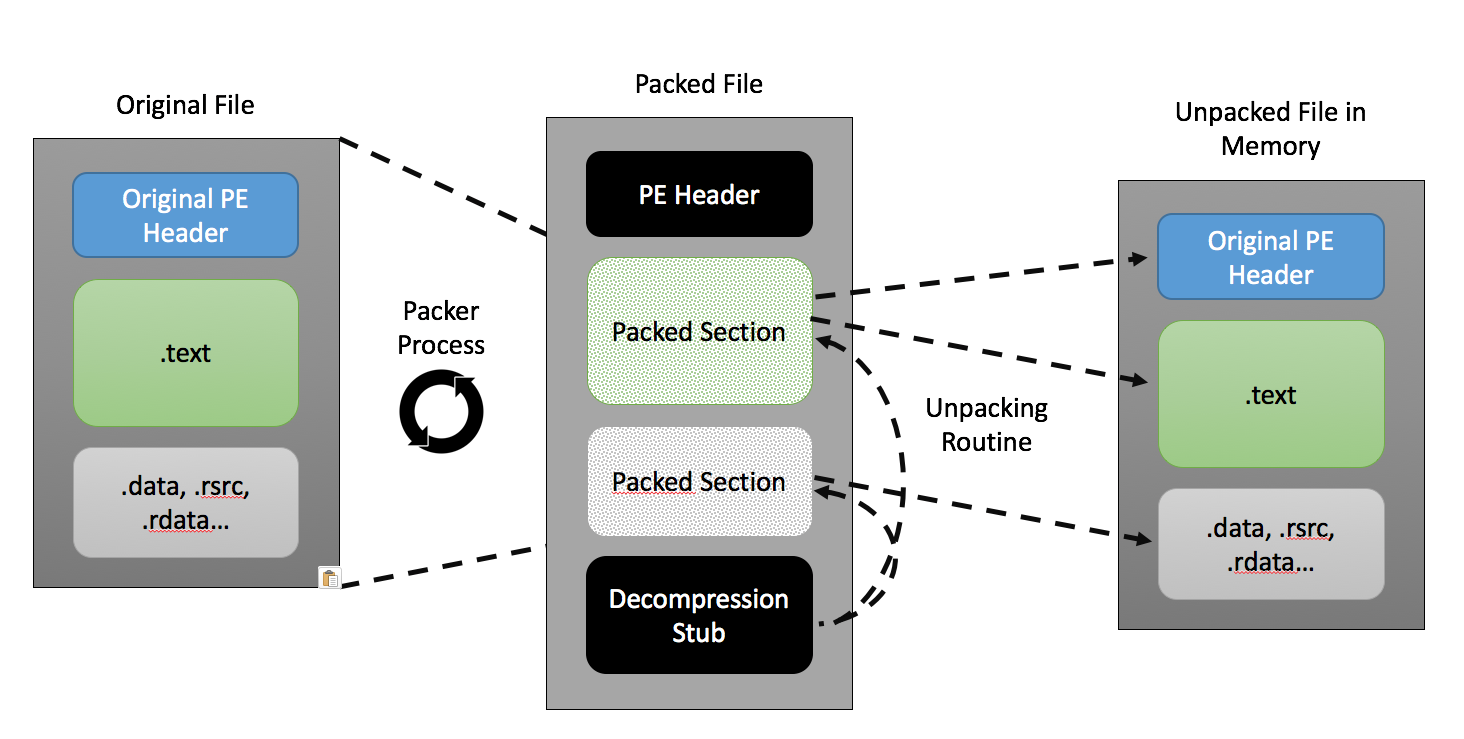
\includegraphics[width=15cm]{Packers.png}
\caption{}
\centering
\end{figure}

U području računalne sigurnosti posebno su učestali packeri za Windows Portable Executable, tj. PE datoteke.

\subsection{Opis problema}

PE datoteke su povijesno najčešći nositelji malicioznog koda u obliku virusa, ransomwarea,
trojanskih konja, itd., te se packeri koriste da bi se taj maliciozni kod prikrio. Klasična statička
analiza (bez pokretanja datoteka) koju provode antivirusi bazira se na potpisima. Oni nastaju
tako da se prikupe primjeri nekog malwarea te se pronađe niz byteova specifičan za taj malware, koji se zatim traži prilikom skeniranja datoteka antivirusom.


\vspace{3mm}


Primjenom packera mijenja se sadržaj datoteke, zbog čega potpisi mogu prestati biti prisutni.
Na taj se način iz jedne maliciozne datoteke može napraviti više različitih inačica. Packeri koji
imaju nemalicioznu primjenu vrlo su rijetki u odnosu na packere koji se koriste za malware.

\subsection{Skup podataka}
S obzirom da rjesavamo problem sa natjecanja Mozgalo, skup podataka za ovaj problem nam je omogucio zlatni partner Mozgala, tvrtka ReversingLabs. Oni su razvili ReversingLabs TitaniumCore\textsuperscript{TM} platformu koja prepoznaje PE packere koriste TitaniumCore potpise koje pišu stručnjaci za reverzno inženjerstvo i analizu sigurnosnih prijetnji.

\vspace{3mm}

Skup podataka bazirat će se na skupu raznovrsnih packera i dodatnim nepakiranim
datotekama. Svaki primjer se sastoji od dva dijela: originalne datoteke i TitaniumCore
izvještaja za tu datoteku.

\section{Cilj i hipoteze istraživanja problema}

Pristup pisanja potpisa za pojedine \textit{packere} je vremenski zahtjevan te zahtjeva vec izdvojene pakiranih datoteka.

Cilj istrazivanja problema je, uz dani skup podataka, napraviti sustav za detekciju pakiranih datoteka.

\vspace{3mm}

Pojedine znacajke unutar TitaniumCore izvjestaja nam daju odredene naznake da bi datoteka mogla biti pakirana, poput imena odjeljaka (\textit{Section name}) i entropije dane datoteke.\\
Primjerice, nekad imena razlicitih odjeljaka nose ime pojedinih packera (UPX), te je entropija pakirane datoteke generalno puno veca nego u obicnim datotekama.\\
No, problem je sto dosta stvari koje se prikazuju u TitaniumCore izvjestaju mogu biti rucno mijenjane u danoj datoteci pa ne mozemo uzeti pojedinu znacajku zdravo za gotovo.\\
Zbog svega navedenoga, hipoteze naseg istrazivanja su:

\begin{itemize}
\item Pojedine znacajke u TitaniumCore reportu su usko vezane uz to je li neka datoteka pakirana ili ne
\item Kombinacijom tih znacajki nadziranim ucenjem, mozemo postici visok rezultat 
\item Prepoznavanje malware kampanja
\item Lakši odabir packera za koje se isplati razvijati unpackere
\end{itemize}

\vspace{3mm}

Metoda automatske detekcije pakiranih datoteka omogucila bi:

\begin{itemize}
\item Izdvajanje zanimljivih malware datoteka za detaljniju analizu
\item Ranu detekciju nikad prije viđenog malwarea
\item Prepoznavanje malware kampanja
\item Lakši odabir packera za koje se isplati razvijati unpackere
\end{itemize}

\section{Pregled dosadašnjih istraživanja}

Analiza entropije se koristi za uvid u sadržaj PE datoteka, primarno za detekciju kompresije i kriptografije tipično vezanih uz \textit{packere}.
Dio pristupa se bazira na analizi svojstava PE zaglavlja i jednostavnim klasifikatorima. Također, znatno poboljšanje točnosti detekcije malwarea dobiveno je koristeći stablo odluke za detekciju pakiranja.

\vspace{3mm}

Radovi koji koriste ovaj pristup kvalitetan su izvor analize značajnosti komponenata PE formata, ali su isto
tako skloni pretreniranju zbog ograničenosti podataka s kojima rade. 


%------------------------------------------------
\iffalse
\subsection{Heading on level 2 (subsection)}

Aenean commodo ligula eget dolor. Aenean massa. Cum sociis natoque penatibus et magnis dis parturient montes, nascetur ridiculus mus. Donec quam felis, ultricies nec, pellentesque eu, pretium quis, sem.

%------------------------------------------------

\subsubsection{Heading on level 3 (subsubsection)}

\lipsum[3] % Dummy text

\paragraph{Heading on level 4 (paragraph)}

\lipsum[6] % Dummy text

%----------------------------------------------------------------------------------------
%	PROBLEM 2
%----------------------------------------------------------------------------------------

\section{Lists}

%------------------------------------------------

\subsection{Example of list (3*itemize)}
\begin{itemize}
	\item First item in a list 
		\begin{itemize}
		\item First item in a list 
			\begin{itemize}
			\item First item in a list 
			\item Second item in a list 
			\end{itemize}
		\item Second item in a list 
		\end{itemize}
	\item Second item in a list 
\end{itemize}

%------------------------------------------------

\subsection{Example of list (enumerate)}
\begin{enumerate}
\item First item in a list 
\item Second item in a list 
\item Third item in a list
\end{enumerate}

%----------------------------------------------------------------------------------------
\fi
\end{document}